\chapter{Analyse des besoins et choix de technologie}

\section{Introduction}

Ce chapitre formalise les besoins fonctionnels et non fonctionnels auxquels doit répondre l'architecture, puis justifie les technologies retenues à travers un état de l'art ciblé. Il aborde successivement les protocoles de communication IoT, les mécanismes de sécurisation des flux (TLS~1.3, mTLS), les infrastructures à clés publiques adaptées à l'IoT, ainsi que les approches de détection (IDS, SIEM, Machine Learning). Une synthèse comparative positionne notre solution par rapport aux travaux et offres existants.

\section{Analyse des besoins}

\subsection{Besoins fonctionnels}

L'analyse a permis d'identifier les besoins fonctionnels suivants, structurés selon les sous-systèmes de l'architecture cible :

\begin{itemize}
  \item \textbf{BF-1 -- PKI dynamique} : émettre, renouveler et révoquer automatiquement des certificats X.509 pour des centaines de dispositifs.
  \item \textbf{BF-2 -- Broker MQTT sécurisé} : accepter uniquement des connexions TLS~1.3 avec authentification mutuelle et appliquer des politiques d'accès par topic.
  \item \textbf{BF-3 -- Simulation de flotte} : reproduire le trafic d'une flotte hétérogène de dispositifs IoT à partir d'un dataset réel multi-classes.
  \item \textbf{BF-4 -- Détection réseau} : analyser le trafic MQTT chiffré et générer des alertes structurées (JSON) pour les comportements suspects.
  \item \textbf{BF-5 -- Centralisation SIEM} : ingérer, corréler et visualiser les alertes de sécurité dans un tableau de bord unifié.
  \item \textbf{BF-6 -- Détection comportementale} : apprendre les profils de communication normaux et signaler statistiquement les déviations via Machine Learning.
\end{itemize}

\subsection{Besoins non fonctionnels}

\begin{table}[H]
\centering
\caption{Besoins non fonctionnels du système}
\label{tab:bnf}
\begin{tabular}{llp{6cm}}
\toprule
\textbf{ID} & \textbf{Catégorie} & \textbf{Exigence} \\
\midrule
BNF-1 & Sécurité & TLS~1.3 obligatoire, mTLS, suites cryptographiques modernes (AES-GCM, ECDHE) \\
BNF-2 & Performance & RTT MQTT $<$ 100~ms, throughput $>$ 1\,000~msg/s, handshake TLS $<$ 200~ms \\
BNF-3 & Reproductibilité & Environnement intégralement simulé sous GNS3, scripts versionnés sous Git \\
BNF-4 & Open source & Composants gratuits et auditables \\
BNF-5 & Observabilité & Journalisation centralisée, alertes structurées, visualisation temps réel \\
BNF-6 & Scalabilité & Support d'au moins 50 dispositifs simultanés en mTLS \\
\bottomrule
\end{tabular}
\end{table}

\section{Protocoles de communication IoT}

\subsection{MQTT -- Message Queuing Telemetry Transport}

MQTT est un protocole de messagerie \textit{publish/subscribe} conçu pour les réseaux à faible bande passante et les dispositifs à ressources limitées. Initialement développé par IBM en 1999, il est devenu la norme \textbf{ISO/IEC~20922:2016} et le standard de facto pour l'IoT industriel~\cite{mqtt5}. Son architecture repose sur trois acteurs : le \textbf{broker} (courtier central), les \textbf{publishers} (émetteurs) et les \textbf{subscribers} (consommateurs). MQTT supporte trois niveaux de qualité de service (\ac{QoS}) : QoS~0 (\textit{at most once}), QoS~1 (\textit{at least once}) et QoS~2 (\textit{exactly once}). Dans notre projet, QoS~1 est utilisé pour l'équilibre fiabilité/performance.

\textbf{Faiblesses natives :} sans configuration explicite, MQTT v3.1.1 transmet les données en clair sur TCP port 1883 et n'effectue aucune vérification d'identité. MQTT~v5 améliore la situation mais ne rend pas TLS obligatoire.

\subsection{Comparatif des protocoles IoT}

\begin{table}[H]
\centering
\caption{Comparatif des principaux protocoles de communication IoT}
\label{tab:protocoles_iot}
\begin{tabular}{lllllp{3.2cm}}
\toprule
\textbf{Protocole} & \textbf{Transport} & \textbf{Modèle} & \textbf{QoS} & \textbf{Sécu. native} & \textbf{Usage typique} \\
\midrule
MQTT~5 & TCP & Pub/Sub & 0-1-2 & TLS optionnel & IoT, télémétrie \\
CoAP & UDP & Req/Resp & Oui & DTLS optionnel & Microcontrôleurs \\
AMQP~1.0 & TCP & Pub/Sub & Oui & TLS + SASL & Entreprise, finance \\
HTTP/2 & TCP & Req/Resp & N/A & TLS (HTTPS) & APIs REST IoT \\
WebSocket & TCP & Full-duplex & N/A & TLS & Dashboards temps-réel \\
\bottomrule
\end{tabular}
\end{table}

Le choix de MQTT pour ce projet est motivé par sa large adoption dans l'écosystème IoT industriel, son faible overhead protocolaire et la disponibilité d'implémentations open source matures (Mosquitto).

\section{Sécurité des flux IoT}

\subsection{Vecteurs d'attaque principaux}

L'ENISA~\cite{enisa_iot} et le MITRE ATT\&CK ICS framework identifient plusieurs catégories d'attaques ciblant les écosystèmes IoT :

\begin{description}
  \item[Interception (MiTM)] Absence de chiffrement ou certificats non vérifiés permettant l'écoute passive ou l'injection active.
  \item[Usurpation d'identité] Connexion au broker avec des identifiants volés ou sans authentification forte.
  \item[DoS / DDoS] Inondation du broker avec des milliers de connexions ou de publications~\cite{kolias2017mirai}.
  \item[Injection de données] Publication de valeurs malveillantes sur les topics de commande pour affecter les actionneurs.
  \item[Replay] Rejeu de messages chiffrés capturés pour déclencher des actions non autorisées.
\end{description}

\subsection{TLS 1.3 et mTLS pour MQTT}

TLS~1.3 (RFC~8446~\cite{rfc8446}, 2018) est la version recommandée pour les connexions MQTT sécurisées. Ses principales avancées par rapport à TLS~1.2 sont :

\begin{itemize}
  \item \textbf{0-RTT resumption} pour les connexions répétées sur même session.
  \item Suppression des algorithmes faibles (RSA key exchange, RC4, MD5/SHA-1).
  \item \textbf{Forward Secrecy} obligatoire via ECDHE.
  \item Handshake réduit à \textbf{1~RTT} contre 2~RTT pour TLS~1.2.
\end{itemize}

Le \textbf{mTLS} (\textit{mutual TLS}) étend le handshake standard en exigeant que le client présente également un certificat signé par la CA de confiance. Cela permet d'authentifier à la fois le serveur \textit{et} le client, ce qui est critique pour des dispositifs IoT dont on veut contrôler l'identité. La figure~\ref{fig:tls_handshake_etat_art} illustre le processus de handshake TLS~1.3 en mode mTLS.

\begin{figure}[H]
  \centering
  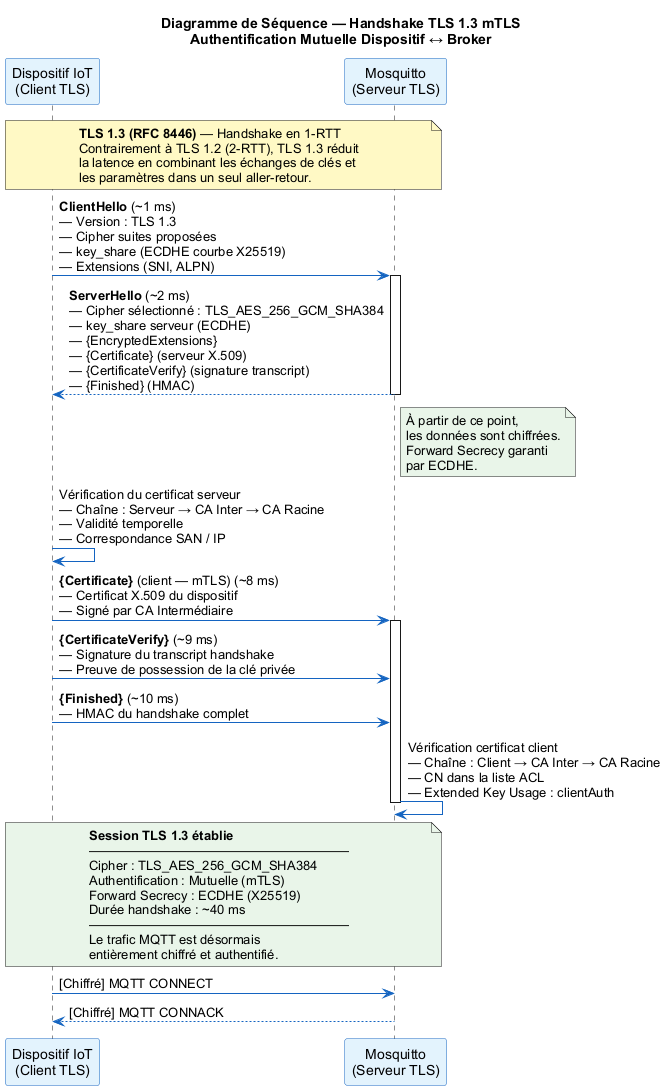
\includegraphics[width=0.7\textwidth]{diagrams/diag-tls-handshake.png}
  \caption{Handshake TLS~1.3 en mode mTLS (diagramme de séquence)}
  \label{fig:tls_handshake_etat_art}
\end{figure}

\section{Infrastructures à clés publiques pour l'IoT}

\subsection{Défis spécifiques}

La gestion des certificats dans un écosystème IoT présente des défis uniques~\cite{nist_sp800213} : volume important de dispositifs, durée de vie courte des certificats pour limiter l'exposition, rotation entièrement automatisée et révocation accessible même sur réseaux contraints.

\subsection{HashiCorp Vault comme PKI dynamique}

HashiCorp Vault est une solution open source de gestion des secrets et de PKI dynamique~\cite{vault_pki}. Son moteur \texttt{pki} permet l'émission automatisée de certificats X.509 via API REST ou CLI, la définition de \textbf{rôles} avec contraintes (TTL, CN autorisés, IP SAN), l'intégration avec des orchestrateurs et la révocation immédiate avec génération automatique de CRL. La figure~\ref{fig:pki_hierarchy_etat_art} présente le modèle de hiérarchie PKI à deux niveaux retenu.

\begin{figure}[H]
  \centering
  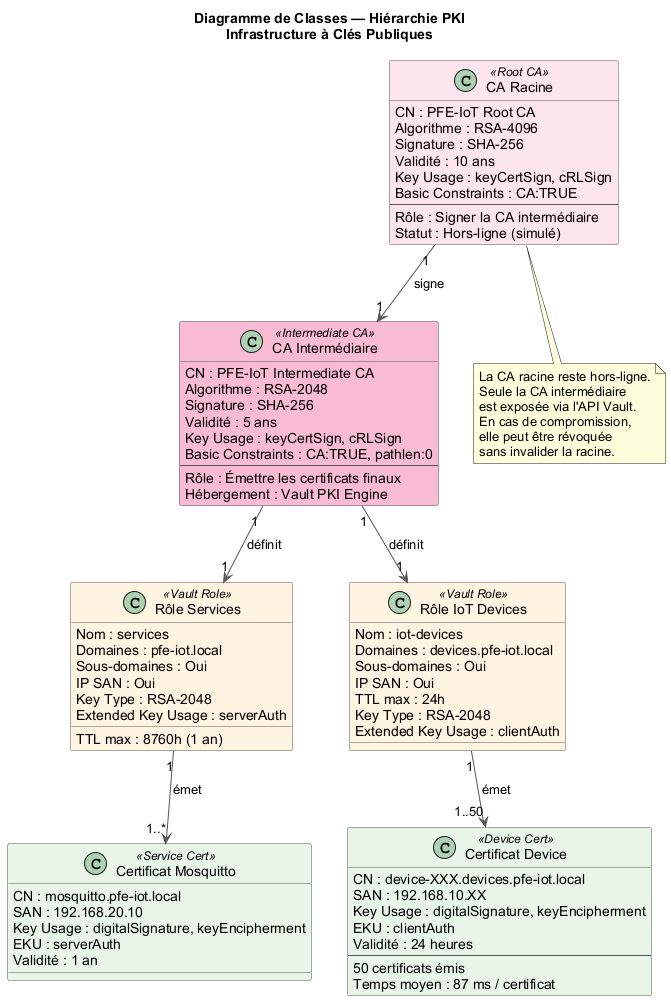
\includegraphics[width=0.75\textwidth]{diagrams/diag-pki-hierarchy.png}
  \caption{Hiérarchie PKI -- diagramme de classes (CA Racine, CA Intermédiaire, Rôles)}
  \label{fig:pki_hierarchy_etat_art}
\end{figure}

\section{Détection d'anomalies, IDS et SIEM}

\textbf{Suricata} est un moteur IDS/IPS open source multi-thread supportant l'inspection en profondeur des paquets (DPI)~\cite{suricata_mqtt}. Il supporte nativement le protocole MQTT depuis sa version 6.0 (\texttt{app-layer-protocol: mqtt}), ce qui permet d'écrire des règles spécifiques aux topics et aux payloads.

\textbf{Wazuh} est une plateforme SIEM open source issue du fork d'OSSEC~\cite{wazuh_docs}. Elle offre un agent léger, un moteur de règles configurable avec corrélation multi-sources, l'intégration native avec OpenSearch pour la visualisation, et des modules spécialisés pour Suricata, Docker et Kubernetes.

\subsection{Machine Learning pour la détection d'anomalies IoT}

Deux approches complémentaires ont été retenues. \textbf{IsolationForest}~\cite{liu2008isolation} est un algorithme non supervisé basé sur la construction d'arbres d'isolation aléatoires : les points anormaux, étant rares et distincts, sont isolés en un nombre minimal de partitions. Son avantage majeur est l'absence de nécessité d'étiquettes : il peut détecter des attaques inconnues. \textbf{Random Forest}~\cite{breiman2001random} est un ensemble d'arbres de décision entraîné en mode supervisé. Il exploite les étiquettes disponibles pour apprendre les signatures spécifiques de chaque type d'attaque, atteignant des performances proches de la perfection sur des datasets équilibrés.

\section{Synthèse et positionnement}

\begin{table}[H]
\centering
\caption{Positionnement par rapport aux solutions et travaux existants}
\label{tab:positionnement}
\begin{tabular}{lcccc}
\toprule
\textbf{Solution} & \textbf{PKI complète} & \textbf{mTLS MQTT} & \textbf{IDS} & \textbf{ML détection} \\
\midrule
AWS IoT Core & \checkmark & \checkmark & $\sim$ & $\sim$ \\
Azure IoT Hub & \checkmark & \checkmark & $\sim$ & \checkmark \\
Eclipse Mosquitto (base) & $\times$ & Optionnel & $\times$ & $\times$ \\
Travaux académiques & Partiel & Partiel & Partiel & Isolé \\
\textbf{Cette architecture} & \checkmark & \checkmark & \checkmark & \checkmark \\
\bottomrule
\end{tabular}
\end{table}

Notre contribution se distingue par l'intégration verticale complète, du certificat dispositif jusqu'à la détection ML, dans un environnement simulé reproductible et entièrement open source. Le tableau~\ref{tab:choix_tech} récapitule les choix technologiques retenus, dont la mise en œuvre concrète est détaillée au chapitre suivant.

\begin{table}[H]
\centering
\caption{Justification des choix technologiques}
\label{tab:choix_tech}
\begin{tabular}{llp{6cm}}
\toprule
\textbf{Composant} & \textbf{Technologie} & \textbf{Justification} \\
\midrule
Simulation réseau & GNS3 & Standard académique, support Docker natif, reproductible \\
Routeur & MikroTik CHR & Utilisé en production chez TT, RouterOS complet \\
Broker MQTT & Mosquitto & Open source, TLS~1.3 natif, ACL avancées \\
PKI & HashiCorp Vault & API programmatique, rotation automatique \\
IDS & Suricata & Support MQTT natif, multi-thread \\
SIEM & Wazuh & OpenSearch intégré, agents légers, gratuit \\
ML & scikit-learn & Large écosystème, IsolationForest + RF disponibles \\
\bottomrule
\end{tabular}
\end{table}

\section{Conclusion}

Ce chapitre a formalisé les besoins fonctionnels et non fonctionnels à couvrir et passé en revue les principales briques technologiques disponibles pour y répondre. Les choix retenus -- MQTT sur TLS~1.3/mTLS, PKI HashiCorp Vault, IDS Suricata, SIEM Wazuh et pipeline ML scikit-learn -- forment une chaîne cohérente, entièrement open source et reproductible. Le chapitre suivant présente la réalisation concrète de cette architecture, depuis la topologie réseau jusqu'au déploiement détaillé de chaque composant.
